\chapter{Implementation}
\label{ch:Implementation}
This chapter explains the detailed implementation of the methods described in \autoref{ch:Methodology}. It covers the specific processes, experiments, and analyses done during the research. This includes the practical steps taken to prepare images, apply distortions, extract features, and train the models to assess image quality in teledermatology. \par

\section{Image Selection and Labeling Process}
\label{sec:ImgSelectLabel}
This section describes the first stages of the implementation, focusing on the selection and preparation of the image datasets used in the research. The images considered for this research were in JPG and PNG formats. \par

\subsection{Image Filtering and Selection}
\label{sub:ImgFilterSelect}
The first step in preparing the images involves carefully selecting good quality images from the SCIN \autocite{SCIN} and Fitzpatrick17k datasets \autocite{F17K}. This manual selection process makes sure that no mistakes are made and only clear images are included in the training set. The focus during selection is on images that are well-framed and free from distortions that could affect their usefulness for making accurate medical diagnoses. \par
\vspace{\baselineskip}
\noindent
Key criteria for selecting good quality images include clarity, proper lighting, and accurate color representation. Clear images are important for accurate diagnosis, as they allow for detailed examination of the skin condition. A good indication of clarity is the visibility of fine details like hair follicles, which shows that the image is not blurry. Proper lighting is also necessary, as it helps in accurately displaying the skin’s condition. Images should neither be too bright nor too dark, as this can hide important details. Balanced contrast, where the light and dark areas of the image are evenly distributed, is important for a clear view of the skin’s texture and color. Accurate color representation is another critical factor. The images must realistically represent skin tones and colors, as this is needed for correct diagnosis. Any change in color can lead to misinterpretation of the skin condition. \par
\vspace{\baselineskip}
\noindent
By carefully filtering and selecting images based on these criteria, the dataset is prepared with good quality images that are appropriate for further analysis and training in the context of teledermatology. \par

\subsection{Labeling of the Test Set}
\label{sub:LabelingTestSet}
The labeling process involves manually scoring 200 images from the SCIN \autocite{SCIN} dataset. Among these 200 images, around 50 are of good quality and are also included in the test set. Each image is scored on a scale from 0 to 1 for each dermatology quality criterion, where 0 indicates no distortion and 1 indicates extreme distortion. A custom Python script\footnote{playground/create\_labels.ipynb} is used for this labeling process. The script displays each image and prompts the user to enter scores for each quality criterion. The collected scores are organized in a structured format and stored in a JSON file for later analysis. This method ensures that each image is consistently and thoroughly evaluated. \par
\vspace{\baselineskip}
\noindent
The labeling is done using an absolute categorical rating method. This method is time-consuming and requires significant effort from the evaluator. Each of the 200 images is scored on 7 different criteria, resulting in a total of 1400 labels. To maintain accuracy and avoid fatigue, the labeling process is spread out over multiple sessions. This careful and methodical approach helps to ensure that the scores are reliable and that each image is evaluated fairly. \par
\vspace{\baselineskip}
\vspace{\baselineskip}
\section{Distortion Types}
\label{sec:DistTypes}
Here, each dermatology quality criteria type is briefly described, highlighting how they simulate different aspects of image degradation: \par
\begin{enumerate}
    \item Lighting:
        \begin{itemize}
            \item \textit{Brighten}: This operation increases the brightness of an image by applying color space transformations and adjustments, enhancing the overall visual intensity.
            \item \textit{Darken}: Similar to the brighten operation but reduces the visual intensity, making the image darker.
        \end{itemize}
    \item Focus:
        \begin{itemize}
            \item \textit{Gaussian blur}: Applies a Gaussian kernel to create a blurred effect, which softens the image by averaging the pixel values.
            \item \textit{Lens blur}: Uses a circular kernel to simulate the effect of a camera lens blur, causing a more uniform blur across the image.
            \item \textit{Motion blur}: Simulates the effect of motion, either from the camera or the subject, by applying a linear blur in a specified direction.
        \end{itemize}
    \item Orientation:
        \begin{itemize}
            \item \textit{Top perspective}: Alters the image to appear as if viewed from a higher angle, distorting the top part of the image.
            \item \textit{Bottom perspective}: Alters the image to appear as if viewed from a lower angle, distorting the bottom part of the image.
            \item \textit{Left perspective}: Alters the image to appear as if viewed from the left side, distorting the left part of the image.
            \item \textit{Right perspective}: Alters the image to appear as if viewed from the right side, distorting the right part of the image.
        \end{itemize}
    \item Color calibration:
        \begin{itemize}
            \item \textit{Color saturation 1}: Adjusts the saturation in the HSV color space, either increasing or decreasing the vividness of the colors.
            \item \textit{Color saturation 2}: Modifies the color channels in the LAB color space to change the saturation levels, affecting the color intensity.
        \end{itemize}
    \item Background:
        \begin{itemize}
            \item \textit{Color Block}: Uses skin segmentation to apply color block artifacts in the background, simulating background distortions and maintaining focus on the skin area.
        \end{itemize}
    \item Resolution:
        \begin{itemize}
            \item \textit{Change Resolution}: Alters the image resolution to simulate low-quality images by downsampling and then upsampling the image.
        \end{itemize}
    \item Field of view:
        \begin{itemize}
            \item \textit{Crop Image}: Crops the image to simulate different levels of field of view, reducing the visible area of the image.
        \end{itemize}
\end{enumerate}
\vspace{\baselineskip}
\noindent
The distortions for Lighting, Focus, and Color Calibration were adapted from the ARNIQA \autocite{ARNIQA} image degradation model, which was inspired by the KADID \autocite{KADID10k} dataset. These distortions originally provided an extensive range of severity levels. The severity levels were modified to better fit real-world distortions commonly encountered in teledermatology. The rest of the distortions were designed based on observations of real-world image quality issues in teledermatology. \par
\vspace{\baselineskip}
\noindent
For the orientation distortion, the perspective of the image is changed to simulate different viewing angles. By tilting, the image appears as if viewed from a higher, lower, left, or right angle, giving the effect that the camera is not perpendicular to the skin. The resolution distortion is done by first downsampling the image to a lower resolution and then upsampling it back to its original size. This process introduces pixelation and a loss of detail, simulating the effect of low-quality images when enlarged. The field of view distortion involves cropping the image from the left corner to reduce the visible area. Normally, in good quality images, the skin lesion is centered. By cropping the left corner, the lesion moves to the bottom right, simulating poor framing or incomplete capture of the lesion area. Lastly, the background distortion involves segmenting the skin from the background and adding color blocks to create a noisy and cluttered background. This simulates real-world situations where the background is not clean, causing issues in image quality. \par

\section{Distortion Implementation Process}
\label{sec:DistProcess}

\begin{figure}[ht]
    \centering
    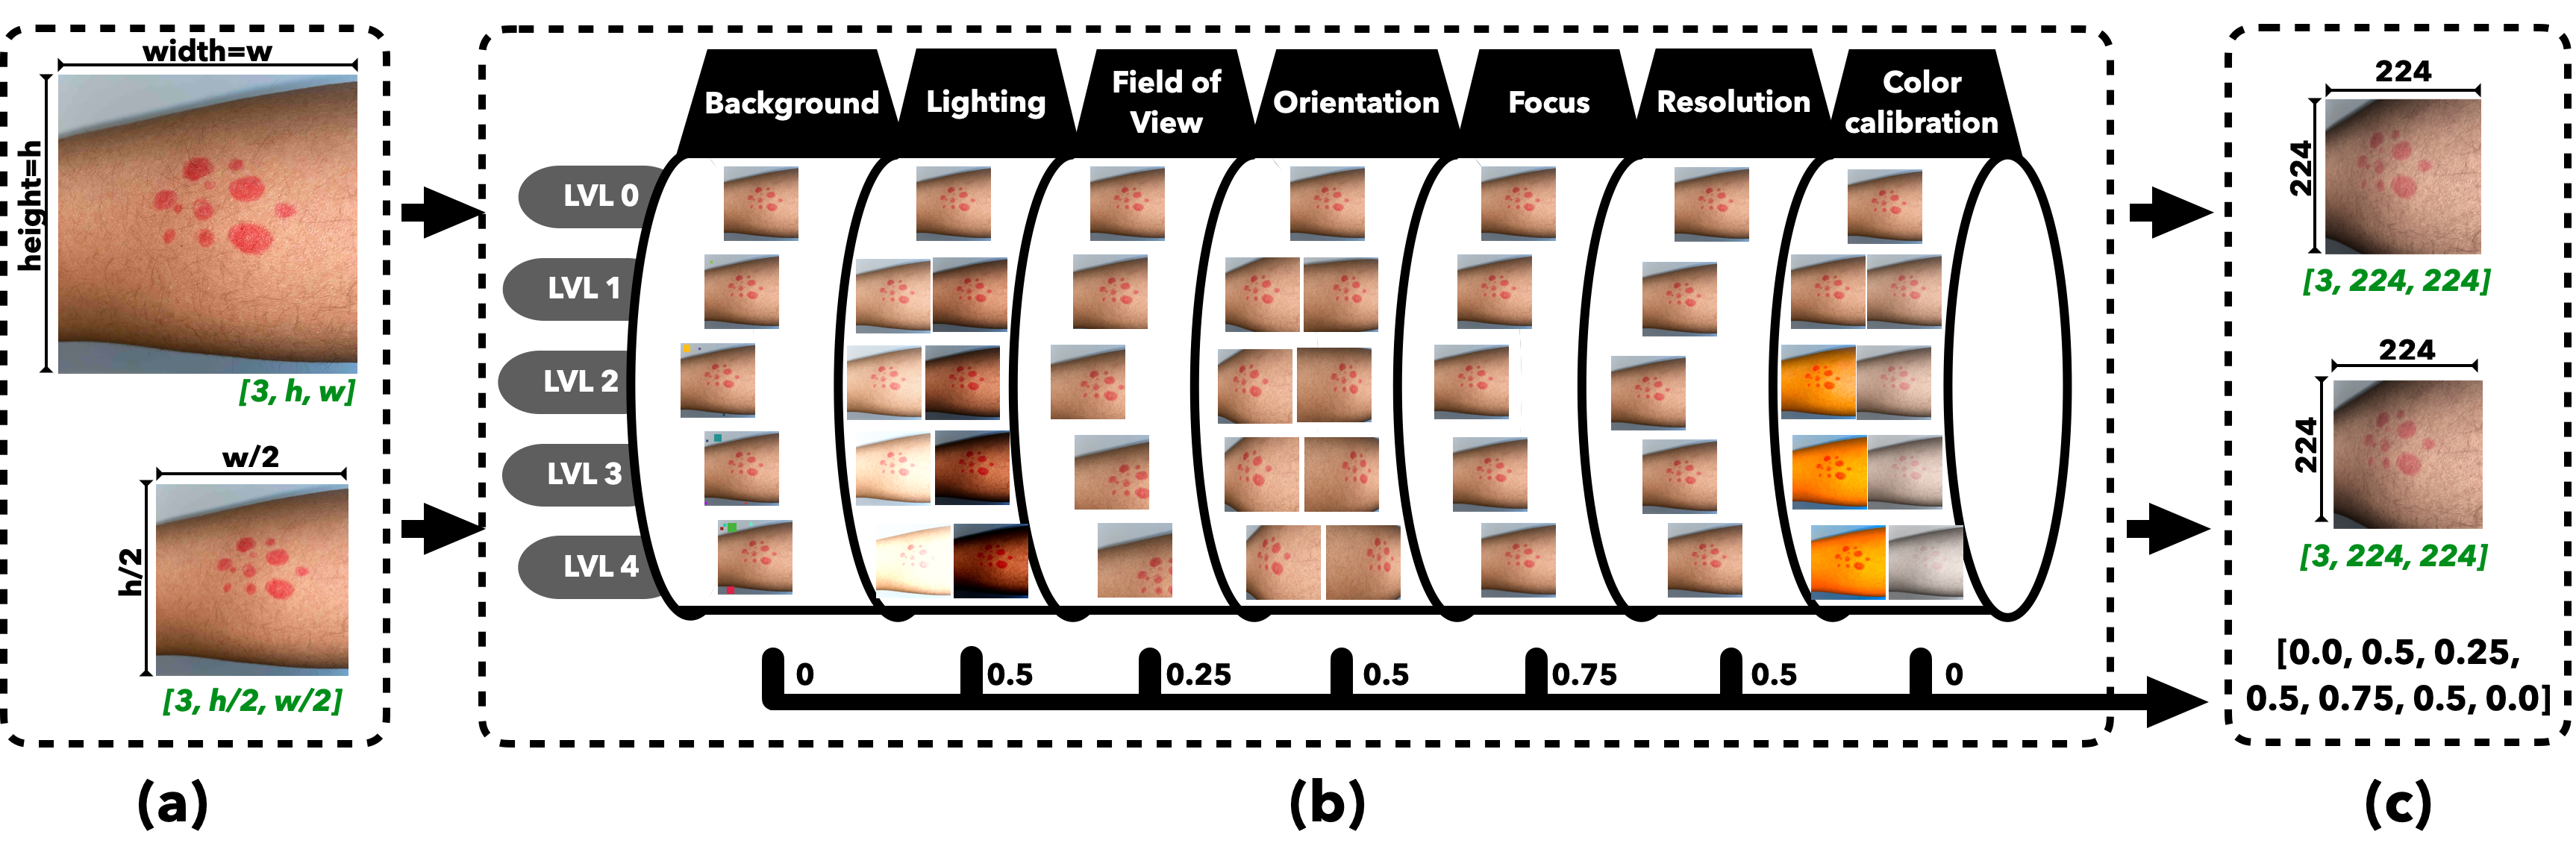
\includegraphics[keepaspectratio,width=15cm]{img/Distortion_pipeline.png}
    \caption{Distortion pipeline for generating training images with different levels of distortion. (a) shows the original image and its downscaled version. (b) shows the distortion pipeline where a type of distortion and a random level for each criterion are selected, with the corresponding mapped values shown at the bottom. (c) shows the output where the distorted original image and the distorted downscaled image are resized to 224x224 pixels, along with the seven distortion values for the image.}
    \label{fig:DistPipeline}
\end{figure}

The distortion implementation process for each dermatology quality criteria involves several key steps to create a range of distorted images, which helps train and evaluate the IQA model.
 \par
\vspace{\baselineskip}
\noindent
For each image, the RGB version is used, and a downsampled version of the image at half the resolution is created. This involves resizing the image to half its original dimensions to simulate lower resolution, following the approach used by ARNIQA’s \autocite{ARNIQA} feature extraction backbone. Distortions are then applied in a specific sequence, as shown in \autoref{fig:DistPipeline}(b). The order matters only for the background distortion, which has to be applied first because it depends on identifying the skin area in the undistorted image. For all other distortions, the order does not matter. If the images have less than 10\% background in proportion to skin, no color blocks are added in the background, and a range value of 0 is used. After that, other distortions are applied based on randomly chosen severity levels. This creates a range of distortion levels across the dataset. \par
\vspace{\baselineskip}
\noindent
Once the distortions are applied, both the original and downsampled images are resized to 224x224 pixels to match the requirements for the backbone. Following resizing, both images are normalized using the mean and standard deviation values of the ImageNet dataset (mean=[0.485, 0.456, 0.406], std=[0.229, 0.224, 0.225]). This normalization ensures the images are processed consistently, as the feature extraction backbone expects the images to have these properties. \par
\vspace{\baselineskip}
\noindent
The severity of each applied distortion is mapped to a value between 0 and 1. This is done because the ranges are, for some distortions, integers and for others, floats in different ranges. Standardizing them, by taking the minimum and maximum possible values of the distortion and scaling the actual distortion value within this range, ensures consistency and maintains the correct ratio of severity across different types of distortions. \par
\vspace{\baselineskip}
\noindent
This process can generate multiple combinations of distorted images because of the random selection of distortion types and severity levels. This significantly increases the number of training images by factors of 4, 8, 16, 32, or 64, though one could experiment with even larger factors. By following this detailed and structured approach, the distortion pipeline effectively simulates a wide range of real-world image quality issues in teledermatology, providing a comprehensive dataset for training and evaluating the image quality assessment model. \par
\vspace{\baselineskip}
\noindent
To make it easier to repeat the experiments, the features and scores from the multiplied images were saved in \textit{.npy} files. These files were named according to the number of distortions, such as \textit{features\_num\_distortions.npy} and \textit{scores\_num\_distortions.npy}. Saving these files means that the exact same sets of distorted images and their related scores can be used again for training and testing different models, allowing for consistent comparisons and evaluations across different tests. By saving these files, there is no need to regenerate the distortions each time, making the experimental process simpler and keeping the evaluation consistent and fair. \par

\clearpage
\section{Feature Extraction with the ARNIQA Backbone}
\label{sec:FeatureExtraction}
After creating the distorted images and their half-scaled versions with mapped labels, the next step is to use the pretrained backbone from ARNIQA \autocite{ARNIQA}, which is loaded via \textit{torch.hub}. This pretrained model has already learned useful features from a large dataset, and these features are transferred to this specific task, a process known as transfer learning. This approach saves time and computational resources. \par
\vspace{\baselineskip}
\noindent
The backbone from ARNIQA generates feature vectors that represent the distortion patterns in the images. By using both the original and downscaled images, the model effectively learns to distinguish between different levels of distortion. This dual-input method provides a comprehensive understanding of image quality variations. \par
\vspace{\baselineskip}
\noindent
The extracted features, which have a shape of (\textit{num\_images}, 4096), represent the learned characteristics of the images. The target labels, indicating distortion severity, have a shape of (\textit{num\_images}, 7) corresponding to the seven distortion criteria. These features and labels are then used to train the final image quality assessment model. \par

\section{Model Training}
\label{sec:ModelTraining}
After expanding the dataset with distorted images, the images were divided into training and validation sets. The training set consisted of 75\% of the images, while the validation set contained the remaining 25\%. This split allowed the models to train on the majority of the data while still having a separate set for evaluating their performance.  \par
\vspace{\baselineskip}
\noindent
Four different multi-output models were experimented with: XGBRegressor, XGBClassifier, MLP Regressor, and MLP Classifier. These models were selected because they can handle complex relationships and predict multiple outputs simultaneously, which is essential for assessing various aspects of image quality. These models were imported from well-established libraries: \textit{xgboost} for XGBRegressor and XGBClassifier, and \textit{sklearn.neural\_network} for MLP Regressor and MLP Classifier. Using these pre-built models has several benefits, including access to optimized and tested implementations, extensive documentation, and community support, which saves time and ensures reliability compared to writing custom models from scratch. \par
\vspace{\baselineskip}
\noindent
Training was conducted using an NVIDIA A16 GPU, equipped with 16GB of vRAM, 1280 CUDA Cores, 40 Tensor Cores, and 512 GB of RAM. This setup made efficient use of resources and sped up the training process. \par
\vspace{\baselineskip}
\noindent
The training involved using the SCIN\textsubscript{distorted}, F17K\textsubscript{distorted}, and COMB\textsubscript{distorted} datasets. Each model was trained individually on these datasets. Additionally, cross-dataset evaluations were conducted to test how well the models generalized across different datasets. For instance, a model trained on SCIN\textsubscript{distorted} was evaluated on F17K\textsubscript{distorted} to assess its robustness and ability to generalize. Combining both datasets and evaluating the models on each dataset individually provided further insights into their performance with a more diverse set of images, ensuring the models did not overfit to a particular dataset. \par
\vspace{\baselineskip}
\noindent
During training, the loss curve was evaluated with early stopping to monitor the model’s performance and prevent overfitting. Early stopping stops the training process if the model’s performance on the validation set does not improve after a certain number of iterations, ensuring the model does not learn noise from the training data. \par

\subsection{Handling Continuous Scores and Discretization}
\label{sub:ContScore}
An important aspect of training the regressors is handling continuous scores. Directly comparing continuous scores to fixed numbers from the distortion pipeline can lead to minor errors. To minimize these errors and accurately calculate metrics like rank correlation and Cohen’s Kappa, the regressor predictions were clipped to the range of 0 to 1 and then categorized into severity levels using a discretization function\footnote{from utils.utils\_data import discretization} that converts continuous scores to discrete categories based on defined thresholds. This process effectively categorizes the severity levels and reduces errors in score comparison.\par
\vspace{\baselineskip}
\noindent
The function ensures that the continuous scores are mapped correctly to discrete categories, providing a standardized way to handle various severity levels. Additionally, the discretization function was used for the classifier models to convert continuous scores to categorical ones, as these models require categorical labels as input. This approach ensured that the models could effectively predict and categorize the severity of distortions in the images. \par

\subsection{Hyperparameter Configuration}
\label{sub:HyperparamConfig}
To find the best hyperparameters, a hyperparameter sweep was performed using Weights and Biases\footnote{\url{https://wandb.ai/site}}. This process involved randomly searching for the best hyperparameters to maximize the overall Spearman’s Rank Order Correlation Coefficient (SRCC). The \autoref{table:mlp_hyperparams} and \autoref{table:xgb_hyperparams} shows the configurations used in the hyperparameter sweep. \par
\vspace{\baselineskip}
\noindent
The hyperparameter sweep aimed to prevent overfitting and help the models perform well on new data. Key parameters were chosen for their ability to control model complexity and improve generalization. \par
\vspace{\baselineskip}
\noindent
The batch size was set to 10 due to hardware limitations. L2 regularization (reg\_lambda) and subsampling (subsample) were used to help the model generalize better. L2 regularization prevents the model from having large coefficients, and subsampling exposes the model to different subsets of data, reducing the chance of overfitting. \par
\begin{table}[ht]
\centering
\begin{tabular}{|l|l|}
\hline
\textbf{MLP Parameter} & \textbf{Sweep Values} \\
\hline
\textit{model\_type} & [mlp\_reg, mlp\_cls] \\
\textit{num\_distortions} & [4, 16, 64] \\
\textit{hidden\_layer\_sizes} & [(512,), (1024,), (512, 256), (1024, 512), (512, 512)] \\
\textit{alpha} & \{"min": 0.0001, "max": 0.01\} \\
\textit{learning\_rate\_init} & \{"min": 0.0001, "max": 0.1\} \\
\textit{max\_iter} & [200, 300, 500] \\
\hline
\textbf{} & \textbf{Fixed Values} \\
\hline
\textit{batch\_size} & 10 \\
\textit{activation} & relu \\
\textit{solver} & adam \\
\textit{early\_stopping} & True \\
\hline
\end{tabular}
\clearpage
\caption{Hyperparameter Configurations for MLP Models}
\label{table:mlp_hyperparams}
\end{table}
\begin{table}[ht]
\centering
\begin{tabular}{|l|l|}
\hline
\textbf{XGB Parameter} & \textbf{Sweep Values} \\
\hline
\textit{model\_type} & [xgb\_reg, xgb\_cls] \\
\textit{num\_distortions} & [4, 16, 64] \\
\textit{n\_estimators} & [50, 100, 200, 300] \\
\textit{learning\_rate} & \{"min": 0.0001, "max": 0.1\} \\
\textit{min\_child\_weight} & \{"min": 1, "max": 150\} \\
\textit{early\_stopping\_rounds} & [10, 20, 30, 40] \\
\textit{subsample} & [0.5, 0.6, 0.7, 0.8, 0.9, 1.0] \\
\textit{max\_depth} & [3, 5, 7, 9] \\
\textit{gamma} & \{"min": 0.001, "max": 0.5\} \\
\textit{multi\_strategy} & [one\_output\_per\_tree, multi\_output\_tree]\\
\hline
\textbf{} & \textbf{Fixed Values} \\
\hline
\textit{batch\_size} & 10 \\
\textit{reg\_alpha} & 0.0 \\
\textit{reg\_lambda} & 1.0 \\
\textit{tree\_method} & hist \\
\textit{objective} & reg:pseudohubererror (specific to XGBRegressor), \\
\textit{} & multi:softprob (specific to XGBClassifier)\\
\textit{n\_jobs} & 16 (specific to XGBRegressor)\\
\textit{booster} & gbtree (specific to XGBClassifier)\\
\textit{eval\_metric} & ['mlogloss', 'merror', 'auc'] (specific to XGBClassifier)\\
\hline
\end{tabular}
\caption{Hyperparameter Configurations for XGB Models}
\label{table:xgb_hyperparams}
\end{table}

\noindent
For the XGB models, the min child weight (min\_child\_weight) parameter was adjusted to make sure each tree leaf had a minimum number of instances, preventing the trees from becoming too complex. The gamma parameter added a constraint on tree growth, which helped to further avoid overfitting by regulating how trees expand during training. \par
\vspace{\baselineskip}
\noindent
By carefully tuning these parameters, the models were designed to balance complexity and generalization, resulting in robust performance on both the training and validation datasets.\par

\subsection{Interpreting Model Performance with Plots}
To understand the models’ performance, several metrics and visual tools were used. Including Mean Absolute Error (MAE), R-squared (R\textsuperscript{2}), Spearman’s Rank Order Correlation Coefficient (SRCC), and Cohen’s Kappa, for each of the seven dermatology quality criteria. These metrics provided detailed insights into where the model performs well and captures distortions effectively and where it does not. An overall score was also calculated to provide a overview of the model’s performance. \par
\vspace{\baselineskip}
\noindent
In addition to numerical metrics, Confusion matrices\footnote{from utils.visualization import plot\_all\_confusion\_matrices} were used for each criterion to show where the model makes correct predictions and where it makes mistakes. These matrices help visualize the accuracy for each type of distortion. They also reveal any biases the model might have, such as predicting only low or high severity levels, or if its predictions are skewed in some way. This detailed view helps identify areas where the model needs improvement and provides insights into its decision-making process. \par

\clearpage
\section{Model Testing}
\label{sec:ModelTesting}
The best model was tested on two specific sets of images to evaluate its performance. The first set, referred to as SCIN\textsubscript{synthetic}, included 70 good quality images that were synthetically distorted using a pipeline to introduce consistent types of distortions. This helped assess how well the model handled controlled distortions. The second set, referred to as SCIN\textsubscript{authentic}, consisted of 200 images with authentic distortions, allowing for a comparison of the model’s performance with human labels. \par
\vspace{\baselineskip}
\noindent
For the SCIN\textsubscript{authentic} images, they were first downscaled to half their size, resized to 224x224 pixels, and normalized. These preprocessed images were then passed through the ARNIQA backbone to extract features, and their actual scores were retrieved from a JSON\footnote{src/test\_200/scores.json} file where the labels were stored. For the SCIN\textsubscript{synthetic} images, the features and scores were saved after extraction from the backbone, and these were stored in a \textit{.npy}\footnote{src/test\_70/embeddings/features.npy} file to allow reproducibility and easier comparison across different tests. \par
\vspace{\baselineskip}
\noindent
To visualize the predictions and test scores, radar charts\footnote{from utils.visualization import plot\_results} were used to observe the model’s strengths and weaknesses across different dermatology quality criteria. For SCIN\textsubscript{synthetic}, a four-column layout was used to present the original image, the distorted image, the actual labels, and the model’s predictions. For SCIN\textsubscript{authentic}, a three-column layout displayed the image, the human-labeled scores, and the model’s predictions. \par

\section{Baseline Comparison}
\label{sec:Baseline}
To evaluate the performance of the proposed image quality assessment model, a baseline comparison was done using both traditional and state-of-the-art methods on the two test sets. The synthetic test set included comparisons with SSIM, ARNIQA, the model’s predictions, and actual scores. The authentic test set included comparisons with ARNIQA, the model’s predictions, and human-labeled scores. This comparison shows how well the proposed model compares to known image quality assessment techniques. \par
\vspace{\baselineskip}
\noindent
Before diving into the details of the individual methods, it is important to understand how the predictions and actual scores were converted into a single quality score. This process makes sure of a consistent and fair comparison. \par
\vspace{\baselineskip}
\noindent
To do this, a weighted average\footnote{playground/create\_labels.ipynb} method was used to give more importance to higher distortion values, which have a bigger effect on overall image quality. The function calculates the average of the seven distortion scores by first creating weights based on how severe each distortion is. This means that higher distortion scores will have a bigger impact on the final quality score. The scores are squared to highlight higher distortion values, and these squared scores are then normalized by dividing each by the sum of all the squared scores. This step makes sure that the weights add up to 1, keeping the balance between the different scores. \par
\vspace{\baselineskip}
\noindent
The function then uses these normalized weights to compute the weighted average of the distortion scores. This results in a single score ranging from 0 to 1, where 0 indicates good quality (no distortion) and 1 indicates poor quality (high distortion). This method makes sure that the final quality score accurately shows the severity of the distortions in the image. \par

\subsection{Traditional Image Quality Assessment (SSIM)}
For the SSIM (Structural Similarity Index) implementation, the SCIN\textsubscript{synthetic} and SCIN\textsubscript{synthetic} ,before distortion, were first converted to RGB format and then resized to 224x224 pixels to match the size used in the model. The SSIM\footnote{src/ssim\_inference.py} was calculated for each pair of images, and the scores were saved in a CSV file for later comparison. \par
\vspace{\baselineskip}
\noindent
It is important to note that SSIM values range from -1 to 1, where 1 indicates perfect similarity, 0 indicates no similarity, and -1 indicates perfect anti-correlation. However, since the quality assessment scores in this research work inversely, with higher values indicating worse quality, the SSIM scores were inverted. This adjustment ensures that the SSIM values can be compared directly to the predicted and actual scores. \par


\subsection{No-Reference  Image Quality Assessment Model (ARNIQA)}
For the ARNIQA\autocite{ARNIQA} implementation, the \textit{single\_image\_inference.py} script from the ARNIQA codebase was referenced and adapted\footnote{src/ARNIQA\_test.py}. The preprocessing steps were done similarly to the model training, involving downscaling, resizing, and normalizing the images. A key difference in this implementation was the need to specify a regressor. ARNIQA provides six different regressors for image evaluation, and for this comparison, the default \textit{KADID10K} regressor was used. Additionally, the \textit{"scale\_score=True"} parameter was set for the model. \par
\vspace{\baselineskip}
\noindent
Similar to the SSIM adjustment, the ARNIQA scores had to be inverted. This is because ARNIQA predicts quality on a scale where 1 indicates good quality and 0 indicates bad quality, which is opposite to the scoring system used in this research. This inversion allows for a direct comparison of ARNIQA scores with the predicted and actual scores from the model. \par
\vspace{\baselineskip}
\noindent
Finally, a line plot was created to compare the different scores from the proposed model, SSIM, and ARNIQA to the actual scores. Additionally, the SRCC values were also calculated to see how well the scores matched the actual quality scores. \par

\subsection{Out of Distribution Testing}
\label{subsec:OOD}
In addition to these comparisons, out-of-distribution testing was done. The script\footnote{src/single\_image\_inference.py} used the same preprocessing and inference steps as in testing the model. This script processes an image and generates a two-column layout, with the image on the left side and a radar chart showing the seven quality criteria for that image on the right side. \par
\vspace{\baselineskip}
\noindent
Different images were chosen from the KADID10K \autocite{KADID10k} dataset, which are different from teledermatology images. For example, images with known distortions such as brightened images were included to check if the model recognizes the brightening, along with color-calibrated images and some good quality images for comparison. This method shows how the model assesses image quality outside its usual teledermatology context. \par
\vspace{\baselineskip}
\noindent
This approach allows for comparing the model’s predictions to see if it identifies distortions correctly. If not, it helps identify limitations, such as difficulties in assessing distortions in general image domains. \par
